\documentclass[a4paper]{article}
\usepackage[brazilian]{babel}
\usepackage{subfig}
\usepackage{booktabs}
\usepackage{graphicx}
%-----------------------------------------------------------------
\title{Projeto 1: C\'{a}lculo da capacidade de suporte {K} do Brasil }
\author{122830 Alcides Goldoni Junior\\
  \small MS 680 - Modelos matem\'{a}ticos aplicados a Biologia\\
  %\small Unicamp 
}%Fechando Title
\begin{document}
\maketitle
%Abstract
%-----------------------------------------------------------------
\abstract{}
%Seções
%-----------------------------------------------------------------
\section{Introdu\c{c}\~{a}o}
Capacidade de suporte ($K$) \'{e} o n\'{u}mero m\'{a}ximo de indiv\'{i}duos que o ambiente pode suportar. Esse conceito, importante em muitas \'{a}reas, \'{e} determinado levando em conta v\'{a}rios fatores como por exemplo: espa\c{c}o, quantidade de alimento, luz, preda\c{c}\~{a}o, entre muitos outros. Esses fatores fazem com que uma esp\'{e}cie cres\c{c}a ou decres\c{c}a em um determinado habitat at\'{e} chegar a um ponto em que ela se estabiliza, variando dentro de um certo limite.
\\
A capacidade de suporte ($K$) \'{e} constante quando as taxas de natalidade e de mortalidade se igualam. Quando uma \'{e} maior ou menor que a outra, a popula\c{c}\~{a}o cresce ou decresce.
\\
Nesse projeto, iremos calcular a capacidade de suporte do Brasil de duas formas diferentes. A primeira, levando considera\c{c}\~{a}o apenas a \'{a}rea do territ\'{o}rio brasileiro e a segunda vamos utilizar os dados de crescimento populacional do IBGE (Instituto Brasileiro de Geografia e Estat\'{i}stica) junto com o modelo de crescimento populacional de Verhulst.
\\
%Começo da sessão de modelos de área%
\section{Modelo 1: Modelo de \'{a}rea}
Para esse modelo, vamos levar em considera\c{c}\~{a}o apenas a \'{a}rea do territ\'{o}rio brasileiro que \'{e} de  8.515.767,049 $km^2$ publicado no Di\'{a}rio Oficial da Uni\~{a}o $n^o$ 118 de 22/06/2016, conforme Resolu\c{c}\~{a}o $N^o$ 02, de 21 de junho de 2016.
\\
Supondo agora que cada brasileiro ocupe dez metros quadrados, ter\'{i}amos uma capacidade de suporte de 8,51E+11 habitantes.
\\
Claro que essa estimativa \'{e} absurda, mas nos serve como valor inicial.
\\
Agora, vamos levar em considera\c{c}\~{a}o a \'area florestal e a \'{a}rea de agricultura. O Brasil det\'{e}m a segunda maior \'{a}rea florestal do planeta com 516 milh\~{o}es de hectares (5,16E+12 $m^2$) aproximadamente 60\% do territ\'{o}rio. J\'{a} as \'{a}reas de cultivo somam 65 milh\~{o}es de hectares (6,50E+11 $m^2$) aproximadamente 31\% do territ\'{o}rio. Dessa forma, temos agora, apenas 9\% do territ\'{o}rio e, portanto, dividindo essa \'{a}rea pelo espa\c{c}o que cada brasileiro ocupa, a capacidade de suporte \'{e} de 2,65E+11 habitantes.
\\
Essa estimativa ainda \'{e} matematicamente poss\'{i}vel mas n\~{a}o faz sentido na realidade.
\\
Sabemos que pessoas n\~{a}o podem permanecer em rodovias, portanto, vamos descontar as estradas e rodovias do pa\'{i}s. Essas, somam 1751868 quil\^{o}metros (1,75E+9 metros). Por padr\~{a}o, para estradas com pista de duas faixas de tr\'{a}fego, a largura da pista \'{e} de 7(sete) metros com 2 (dois) metros de acostamento (seria \'{o}timo se as normas fossem seguidas). Dessa forma, podemos estimar que 2 metros de acostamento mais 7 metros de faixa vezes 1751868 quil\^{o}metros de estrada vezes 2 (faixa de ida e faixa de volta) dando um total de 3,15E+10 metros quadrados de estradas e rodovias. Refazendo os c\'{a}lculos, a capacidade de suporte \'{e} de 2,62E+11 habitantes. 
\\
%essa parte fala dos rios, talvez não seja uma boa fazer isso%
%Vamos levar em considera\c{c}\~{a}o que n\~{a}o podemos morar ou viver sobre as \'{a}guas, dessa forma, vamos descontar as bacias hidrogr\'{a}ficas, essas somam aproximadamente 7,3 milh\~{o}es de quil\^{o}metros quadrados (7,3E+6). Tirando essa valor do territ\'{o}rio que tinhamos, vamos encontrar uma nova capacidade de suporte de \_\_\_\_\_\_\_\_
%finalizado
\\
No come\c{c}o dessas contas, fizemos a suposi\c{c}\~{a}o de que cada brasileiro ocupava dez metros quadrados, sendo essa uma estivativa bem ruim. Utilizando dados da regi\~{a}o sudeste, a mais populosa do pa\'{i}s, temos que a densidade demogr\'{a}fica \'{e} de 160 habitantes por quil\^{o}metro quadrado (Censo 2010). Agora podemos ter uma aproxima\c{c}\~{a}o um pouco melhor e encontrar uma capacidade de suporte de 420E+6 (420 milh\~{o}es) de habitantes.
\\
Podemos melhorar essa estimativa ainda mais. Podemos ver a densidade demogr\'{a}fica no ano de 2010 na tabela \ref{tabelaCensoDem2010}.
\\
\begin{table}[ht!]
\centering
\caption{Densidade demogr\'{a}fica por estado (CENSO 2010)}
\label{tabelaCensoDem2010}
\begin{tabular}{c|c|c}
Regi\~{a}o		&	Estado				&	Densidade demogr\'{a}fica\\
\hline
Norte		&	Rond\^{o}nia		& 	6.58		\\
Norte		&	Acre			&	4.47		\\
Norte		&	Amazonas 		&	2.23		\\
Norte		&	Roraima			&	2.01		\\
Norte		&	Par\'{a} 		&	6.07		\\
Norte		&	Amap\'{a}		&	4.69		\\
Norte		&	Tocantins		&	4.98		\\
Nordeste	&	Maranh\~{a}o 		&	19.81 		\\
Nordeste	&	Piau			&	12.40		\\
Nordeste	&	Cear\'{a}		&	56.76 		\\
Nordeste	&	Rio Grande do Norte	&	59.99 		\\
Nordeste	&	Para\'{i}ba		&	66.70 		\\
Nordeste	&	Pernambuco		&	89.63 		\\
Nordeste	&	Alagoas			&	112.33		\\
Nordeste	&	Sergipe			&	94.35		\\
Nordeste	&	Bahia			&	24.82		\\
Sudeste		&	Minas Gerais		&	33.41 		\\
Sudeste		&	Esp\'{i}rito Santo	&	76.25 		\\
Sudeste		&	Rio de Janeiro		&	365.23  	\\
Sudeste		&	S\~{a}o Paulo		&	166.25  	\\
Sul		&	Paran\'{a}		&	52.40		\\
Sul		&	Santa Catarina		&	65.29		\\
Sul		&	Rio Grande do Sul	&	39.79		\\	
Centro Oeste	& 	Mato Grosso do Sul	&	6.86   		\\
Centro Oeste	& 	Mato Grosso		&	3.36   		\\
Centro Oeste	& 	Goi\'{a}s		&	17.65  		\\
Centro Oeste	& 	Distrito Federal	&	444.07	
\end{tabular}
\end{table}
\\
Com os dados da tabela \ref{tabelaCensoDem2010}, podemos fazer a m\'{e}dia da densidade demogr\'{a}fica obtendo aproximadamente 33 habitantes por quil\^{o}metro quadrado. Dessa forma, encontramos a capacidade de suporte de 86,5E+6 (86,5 milh\~{o}es) habitantes mas capacidade de suporte j\'{a} foi superada, pois hoje temos mais de 200 milh\~{o}es de habitantes e n\~{a}o podemos consider\'{a}-la correta. 
\\
Portanto, para o modelo de \'{a}rea, a capacidade de suporte encontrada \'{e} de 420 milh\~{o}es de habitantes.
\\ 
%Aqui começa o modelo de verhulst
\section{Modelo 2: Verhulst}
Para esse modelo, vamos levar em considera\c{c}\~{a}o o crescimento populacional de acordo com os dados do IBGE e utilzando do modelo de Verhulst estimar a capacidade de suporte ($K$).
\\
Pierre Fran\c{c}ois Verhulst (1804 - 1849) foi um  matem\'{a}tico belga doutor em teoria dos n\'{u}meros. Seu modelo de crescimento populacional foi proposto em 1838, baseado na avalia\c{c}\~{a}o de estat\'{i}sticas dispon\'{i}veis e complementada a teoria do crescimento exponencial com termos representando os fatores de inibi\c{c}\~{a}o de cresimento. A equa\c{c}\~{a}o proposta por Verhulst \'{e}:
%Equação do modelo 
\begin{equation}
\frac{dP}{dt}= \lambda P(1 - \frac{P}{K})
\end{equation}
%Fim da equação do modelo
\\
Onde $\lambda$ \'{e} a taxa de crescimento intr\'{i}nseca, $P$ a popula\c{c}\~{a}o no instante $t$ e $K$ \'{e} a capacidade de suporte do meio, no nosso caso, capacidade de suporte do Brasil.
\\
Utilizando dados do IBGE montamos a tabela e o gr\'{a}fico da figura 1 com o n\'{u}mero de habitantes no Brasil a partir de 1872. 
\begin{figure}[h]
\label{fig_populacao}
\caption{Popula\c{c}\~{a}o residente no pa\'{i}s}
\centering
\subfloat[Gr\'{a}fico de popula\c{c}\~{a}o]{
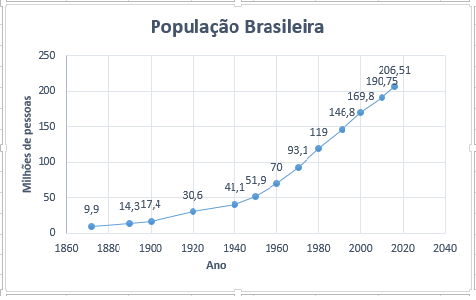
\includegraphics[width=0.6\linewidth]{populacao.png}
}
\subfloat[Tabela de popula\c{c}\~{a}o]{
\label{tabelaPopEvol}
\begin{tabular}{c|c}
Ano		&	Popula\c{c}\~{a}o(em milh\~{o}es)	\\
\hline
1872	&	9,9	\\
1890	& 	14,3	\\
1900	&	17,4	\\
1920	&	30,6	\\
1940	& 	41,1	\\
1950	&	51,9	\\
1960	&	70,0	\\
1970	&	93,1	\\
1980	&	119,0	\\
1990	&	146,8	\\
2000	&	169,8	\\
2010	&	190,8	\\
2016	&	206,5	\\
\end{tabular}
}
\end{figure}
\\
A figura 2 representa o crescimento da popula\c{c}\~{a}o no per\'{i}odo de 1872 a 2016.
\\ 
\begin{figure}[h]
\label{fig_tax_cresc}
\caption{Taxa de crescimento da popula\c{c}\~{a}o}
%\centering
\subfloat[Gr\'{a}fico de crescimento da popula\c{c}\~{a}o]{
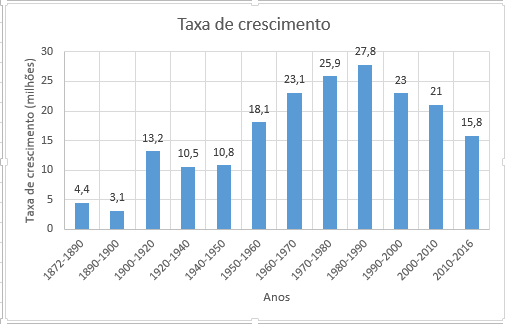
\includegraphics[width=0.6\linewidth]{taxaPopo.png}
}
\subfloat[Tabela crescimento da popula\c{c}\~{a}o]{
\label{tabelaCrescPop}
\begin{tabular}{c|c}
Ano		&	Crescimento da Popula\c{c}\~{a}o(em milh\~{o}es)	\\
\hline
1872-1890	&	4,4   \\
1890-1900	& 	3,1   \\
1900-1920	&	13,2   \\
1920-1940	&	10,5   \\
1940-1950	& 	10,8   \\
1950-1960	&	18,1   \\
1960-1970	&	23,1   \\
1970-1980	&	25,9   \\
1980-1990	&	27,8	\\
1990-2000	&	23,0	\\
2000-2010	&	21,0	\\
2010-2016	&	15,8	\\
\end{tabular}
}
\end{figure}
\\
\\
Com esses dados e utilizando o modelo proposto por Verhulst, vamos calcular a capacidade de suporte utilizando as seguintes equa\c{c}\~{o}es:
\begin{equation}
P_n_+_1 - P_n = \lambda P_n(1 - \frac{P_n}{K})
\end{equation}
Podemos chamar \Delta $P = P_n_+_1 - P_n$ e a equa\c{c}\~{a}o fica:
\begin{equation}
\Delta P  = \lambda P_n(1 - \frac{P_n}{K})
\end{equation}
\\
\begin{equation}
P_n_+_1 - P_n = \lambda  \frac{\lambda}{K}P_n
\end{equation}
\\
Podemos chamar \Delta $P = P_n_+_1 - P_n$ e a equa\c{c}\~{a}o fica:
\begin{equation}
\Delta P = \lambda  \frac{\lambda}{K}P_n
\end{equation}
\\
Com essas equa\c{c}\~{o}es podemos plotar os gr\'{a}ficos de $\frac{\Delta P_n}{P_n}$ x $P_n$ e $\Delta P$ x $P_n$
\\
\begin{figure}[h]
\label{grafLinear}
\caption{Gr\'{a}ficos linear e quadr\'{a}tico para determinar $K$}
%\centering
\subfloat[Gr\'{a}fico de aproxima\c{c}\~{a}o linear]{
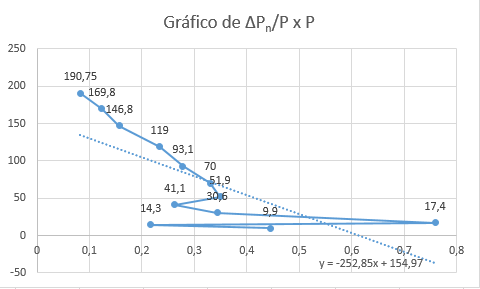
\includegraphics[width=0.5\linewidth]{aproxLin.png}
}
\subfloat[Gr\'{a}fico de aproxima\c{c}\~{a}o Quadr\'{a}tico]{
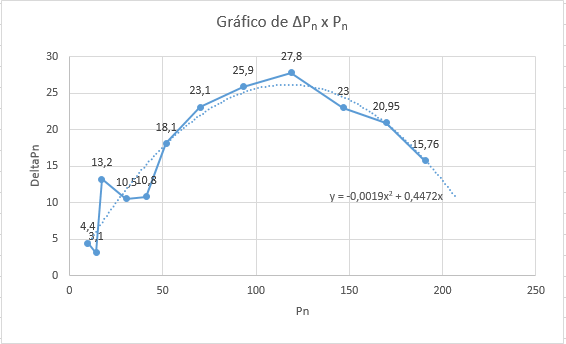
\includegraphics[width=0.5\linewidth]{aproxParab.png}
}
\end{figure}
\\
Pelo gr\'{a}fico de aproximac\~{a}o linear, a equa\c{c}\~{a}o que melhor representa o represente \'{e}:
\begin{equation}
y = -252,85x +154,97
\end{equation}
\\
Assim, podemos ver que a capacidade de suporte \'{e} de aproximadamente 154 milh\~{o}es de habitantes.
\\
Pelo gr\'{a}fico de aproximac\~{a}o quadr\'{a}tica, a equa\c{c}\~{a}o que melhor representa o represente \'{e}:
\begin{equation}
y = - 0,0019x^2 + 0,4472x
\end{equation}
Assim, podemos ver que a capacidade de suporte \'{e} de aproximadamente 235 milh\~{o}es de habitantes.
\\
\section{Conclus\~{a}o}
\\
Atrav\'{e}s dos modelos utilizados nesse projeto, encontramos tr\^{e}s capacidades de suporte diferentes. Dos valores encontrados, aquele que mais se aproxima da realidade \'{e} o modelo de Verhulst com aproxima\c{c}\~{a}o quadr\'{a}tica pois o modelo que leva em considera\c{c}\~{a}o apenas a \'{a}rea \'{e} muito simples e n\~{a}o inclui fatores como \'{a}reas de parques industriais, \'{a}reas fluviais e entre outros fatores que influenciam o tamanho da \'{a}rea "habit\'{a}vel". O modelo de Verhulst com aproxima\c{c}\~{a}o linear tamb\'{e}m n\~{a}o t\~{a}o bom pois a capacidade de suporte que ele nos deu j\'{a} foi ultrapassada e a popula\c{c}\~{a}o continua crescendo e n\~{a}o oscila ao redor daquela capacidade de suporte.


% Bibliografia
%-----------------------------------------------------------------
\begin{thebibliography}{99}
\bibitem {Cd94} http://www.ibge.gov.br/home/geociencias/cartografia/default\_territ\_area.shtm
\bibitem{Cd94} http://www.brasil.gov.br/meio-ambiente/2012/12/brasil-detem-segunda-maior-area-florestal-do-planeta 
\bibitem{Cd94} https://pt.wikipedia.org/wiki/Agricultura\_no\_Brasil
\bibitem{Cd94} https://pt.wikipedia.org/wiki/Transporte\_rodoviario\_no\_Brasil
\bibitem{Cd94} http://www.dnit.gov.br/download/rodovias/operacoes-rodoviarias/faixa-de-dominio/normas-projeto-estr-rod-reeditado-1973.pdf
\bibitem{Cd94} http://www.censo2010.ibge.gov.br/sinopse/index.php?dados=10\&uf=00
\bibitem{Cd94} http://www.suapesquisa.com/geografia/bacias\_hidrograficas.htm
\bibitem{Cd94} http://g1.globo.com/brasil/noticia/2011/04/ibge-atualiza-dados-do-censo-e-diz-que-brasil-tem-190755799-habitantes.html 
\end{thebibliography}

\end{document}
